\section{Results}
\label{sec:experimental_results_tist}

\begin{table}[t]
\centering

% @{}lccccccc@{}
%\begin{tabular}{lm{1.3cm}m{1.3cm}m{1.3cm}m{1.3cm}m{1.3cm}m{1.3cm}m{1.3cm}}
\begin{tabular}{lm{1.3cm}*{7}{>{\centering\arraybackslash}m{1.3cm}}}
\toprule
Modality & \multicolumn{2}{c}{\footnotesize{Cataract Surgery}} & \multicolumn{2}{c}{\footnotesize{OCT}} & \multicolumn{2}{c}{\footnotesize{MRI}} & \multicolumn{1}{l}{\multirow{2}{*}{\footnotesize{Avg. Rel.}}} \\ \cmidrule(lr){2-3}\cmidrule(lr){4-5}\cmidrule(lr){6-7}
Network & \footnotesize{DLV3+} & \footnotesize{scSENet} & \footnotesize{DLV3+} & \footnotesize{scSENet} & \footnotesize{DLV3+} & \footnotesize{scSENet} &   \\ \midrule
Supervised & 15.42 & 37.67 & 22.87 & 24.08 & 52.39 & 65.93 & N/A \\
$\Uppi$ Model~\cite{TESSL} & 27.55 & 35.56 & 1.12 & 0.00 & 10.00 & 6.87 & -22.88 \\
TE~\cite{TESSL} & 33.10 & 42.32 & 42.13 & 39.86 & 63.41 & 67.25 & 11.62 \\
Mean Teacher~\cite{UDAMIS} & 11.06 & 39.54 & 19.11 & 4.70 & 64.82 & 66.87 & -2.04 \\
RL~\cite{Reciprocal} & 34.40 & 45.13 & 48.73 & 47.70 & 60.79 & 70.20 & 14.77 \\
CPS~\cite{CPS} & 36.24 & 39.40 & 47.31 & 14.71 & 76.00 & 68.80 & 10.68 \\
ST~\cite{st++} & 34.34 & 41.10 & 36.84 & 33.01 & 68.63 & 71.97 & 11.26 \\\midrule
% ST++~\cite{st++} &  &  &  &  &  &  &  \\
{\bf TI-ST} & 37.69 & 45.31 & 50.93 & 40.87 & 66.56 & 74.07 & 16.18 \\ 
& \textcolor{gray}{\scriptsize{(+22.27)}} & \textcolor{gray}{\scriptsize{(+7.46)}} & \textcolor{gray}{\scriptsize{(+28.06)}} & \textcolor{gray}{\scriptsize{(+16.79)}} & \textcolor{gray}{\scriptsize{(+14.17)}} & \textcolor{gray}{\scriptsize{(+8.14)}}\\
\bottomrule
\end{tabular}
\sidecaption{Quantitative comparisons in Dice score (\%) among the proposed (TI-ST) and alternative methods for DeepLabV3+~\cite{DeepLabV3} (DLV3+) and scSENet~\cite{SCSE} and the three datasets. Relative Dice computed over the Supervised baseline. \label{tab:quantitative}}


\end{table}


\Cref{tab:quantitative} lists the performance of our transformation-invariant self-training (TI-ST) approach with alternative methods across the three tasks and using two network architectures. According to the quantitative results, TI-ST, RL, ST, and CPS are the best-performing methods. Nevertheless, our proposed TI-ST achieves the highest average relative improvement in dice score compared to naive supervised learning ($16.18\%$ average improvement). Considering our main competitor (RL), we note that our proposed TI-ST method is a one-stage framework using one network. In contrast, RL is a two-stage framework (requiring a pre-training stage) and uses a teacher-student network. Hence, TI-ST is also more efficient than RL in terms of time and computation.  Furthermore, the proposed strategy demonstrates the most consistent results when evaluated on different tasks, regardless of the utilized neural network architecture. 

\textfig{1}{figures/tist_ablation.pdf}{Ablation studies on the pseudo-labeling threshold and size of the labeled dataset.}{fig:tist_ablation}

\Cref{fig:tist_ablation}-(a-b) demonstrates the effect of the pseudo-labeling threshold on TI-ST performance compared with regular ST. We observe that filtering out unreliable pseudo-labels based on transformation variance can remarkably boost pseudo-supervision performance regardless of the threshold. \Cref{fig:tist_ablation}-(c) compares the performance of the supervised baseline, ST, and TI-ST with respect to the number of source-domain labeled training images. While ST performance converges when the number of labeled images increases, our TI-ST pushes decision boundaries toward the target domain dataset by avoiding training with transformation variant pseudo-labels. We validate the stability of TI-ST vs. ST  with different labeling thresholds ($0.80$ and $0.85$) over four training folds in \Cref{fig:ablation_stability}, where TI-ST achieves a higher average improvement relative to supervised learning for different tasks and network architectures. This analysis also shows that the performance of ST is sensitive to the pseudo-labeling threshold and generally degrades by reducing the threshold due to resulting in wrong pseudo labels. However, TI-ST can effectively ignore false predictions in lower thresholds and take advantage of a higher amount of correct pseudo labels. This superior performance is depicted qualitatively in \Cref{fig:qualitative}.


\textfig{1}{figures/ablation_stability.pdf}{Ablation study on the performance stability of TI-ST vs. ST across the different experimental segmentation tasks.}{fig:ablation_stability}

%\begin{figure}[t]
%\centering
%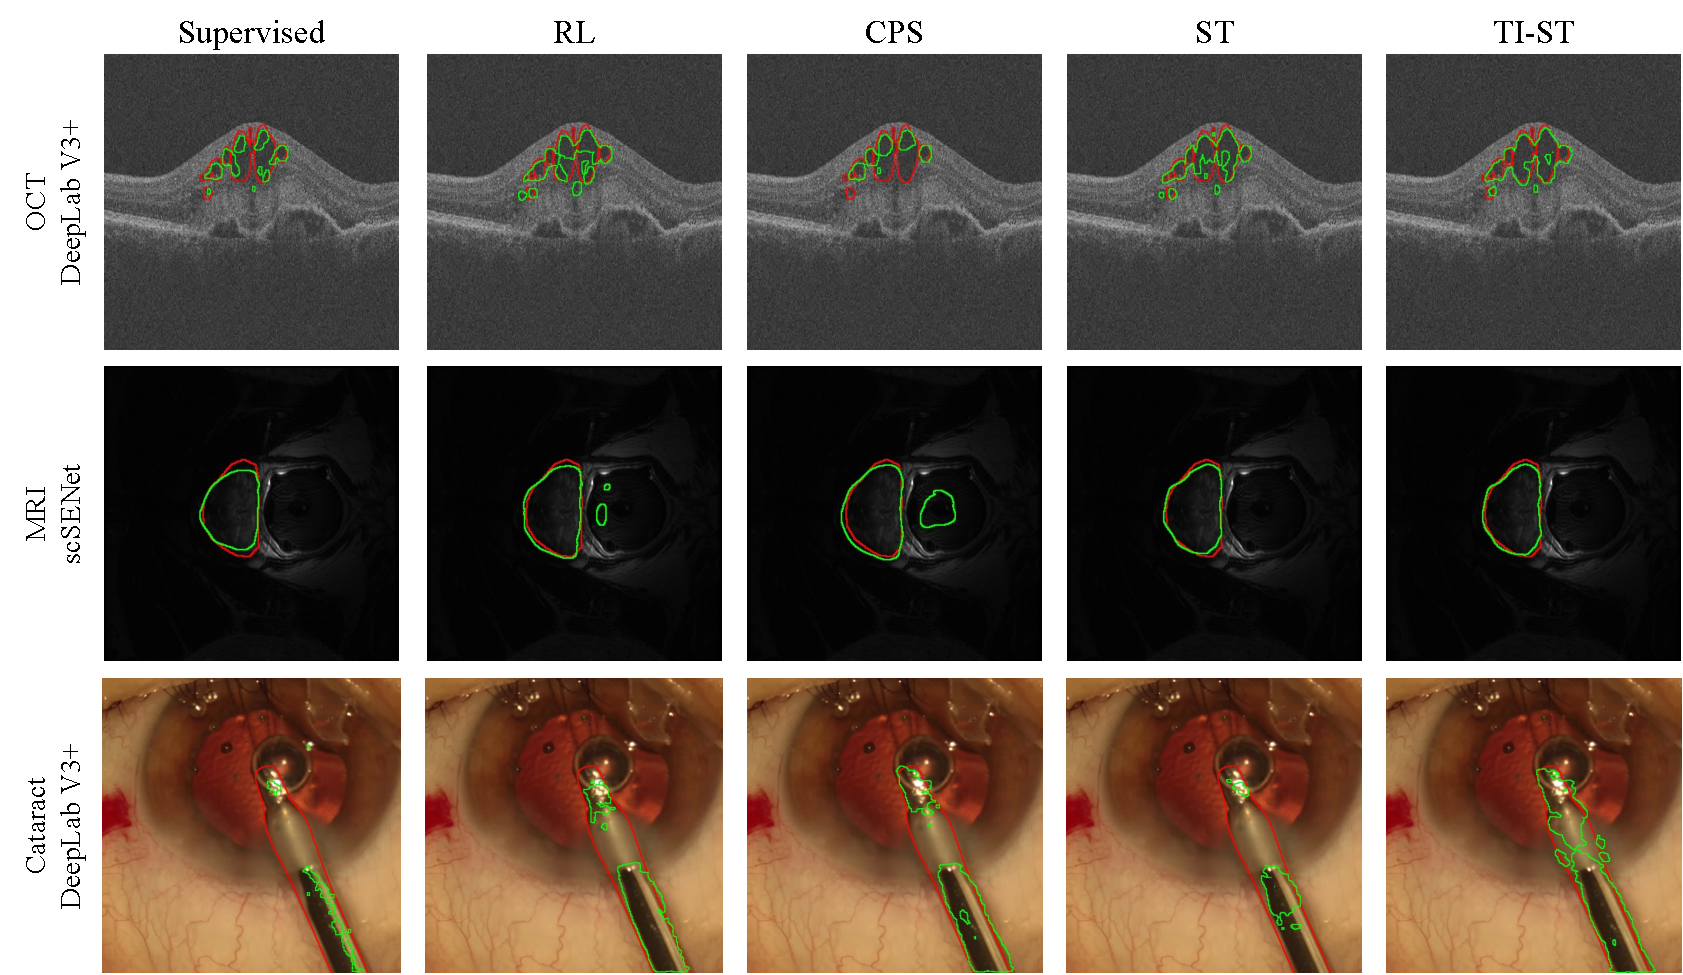
\includegraphics[width=.9\textwidth]{figures/qualitative.pdf}
%\caption{Qualitative comparisons between the performance of TI-ST and four existing methods.
%}
%\label{fig:qualitative}
%\end{figure}
\widefig{1}{figures/qualitative.pdf}{Qualitative comparisons between the performance of TI-ST and four existing methods.}{fig:qualitative}